	\subsection{Robustheit und Pufferung}\label{sec:robustheit}
	Wie wir vorangegangen festgestellt haben, sind einige der Mechanismen, die wir implementieren wollen anfällig gegenüber qualitativ niedrigwertigen Kinectdaten. Tests mit der Kinect haben folgende kritische Situtationen ergeben:
	\begin{itemize}
		\item \textbf{Gelenke und Skelettbestandteile in der Nähe von Objekten und anderen Personen.} Diese können falsch oder verzerrt erkannt werden. So kann etwa die erkannte Handposition zwischen zwei Kinectframes Raumunterschiede von mehreren Metern aufweisen und zurückspringen. Dies kann auch Körperteile betreffen, die vor oder hinter anderen Körperteilen liegen. Für hinter Körpern oder Objekten versteckte Teile ist klar, dass diese von der Kinect nur geraten werden können. Gliedmaßen, die sich vor Körpern (seltener Gegenständen) befinden können durch die Kinect-Optik zum Teil nicht hinreichend von den weiter hinten befindlichen Körperregionen differenziert weren. Das Problem verschärft sich mit zunehmender optischer und räumlicher Ähnlichkeit (Rückstrahlverhalten im sichtbaren Licht und Infrarotlicht sowie annähernd gleiche Entfernung zur Kamera). Ferner steigt die Ungenauigkeit, je weiter man vom \glqq perfekten Abdeckbereich\grqq{} der Kinect entfernt ist.
		\item \textbf{Status der Hände.} Auch bei durchgängiger Aufrechterhaltung eines Handzustands kann es passieren, dass die Kinect vereinzelt falsche Zuweisungen trifft oder keine Zuweisung möglich ist. Besonders schlecht wird die Erkennung, wenn sich die Hände vor dem Körper befinden. Sind die Hände selbst vollständig oder auch nur teilweise verdeckt, ist selbstverständlich ebenfalls keine sinnvolle Erkennung des Handstatus möglich. Hier liegen weitestgehend dieselben Mechanismen zugrunde, die auch die Probleme von Punkt eins verursachen.  
		\item \textbf{Jitterfehler.} Die Kinectdaten sind verrauscht und weisen bspw. von Frame zu Frame kleine Ungenauigkeiten und Abweichungen der Gelenkpositionen in beliebige Richtungen auf. Diese Fehler nehmen ebenfalls umgekehrt Proportional zur Kinect-Sicherheit zu, d.\,h. treten vermehrt auf, wenn die genaue Position nicht richtig erkannt wird und ein \glqq Rateeinfluss\grqq{} vorhanden ist. Insbesondere ist dies wieder bei Verdeckung (egal in welcher Reihenfolge) mit optischer und räumlicher Nähe der Fall. Dieser Punkt sei jedoch von Fehlern nach Punkt eins insofern abgegrenzt, dass wir uns hier auf ständig auftretende, von ihrer Natur her kleine Fehler beziehen, obwohl Punkt eins natürlich auch bewirken kann, dass die Kinectdaten in beliebige Richtungen \glqq zittern\grqq{}.
		\item \textbf{Phantome.} Mitunter kann es passieren, dass ein ganzes Skelett an einem Gegenstand hängenbleibt. Dies geschieht, wenn eine getrackte Person einen Gegenstand passiert und dabei nicht korrekt erkannt wird -- etwa weil sich die Situation sehr nahe am Rand des Aufnahmebereichs abspielt oder der Gegenstand eine nahezu humanoide Form hat. Sobald die Person wieder richtig erkannt wird, erhält sie ein neues Skelett. Die Skelettdaten dieser Phantome sind dann abgesehen von der Orientierung an menschenähnlichen Merkmalen komplett geraten und variieren über die Zeit sehr stark und willkürlich.
	\end{itemize}
	\begin{figure}
	\centering
	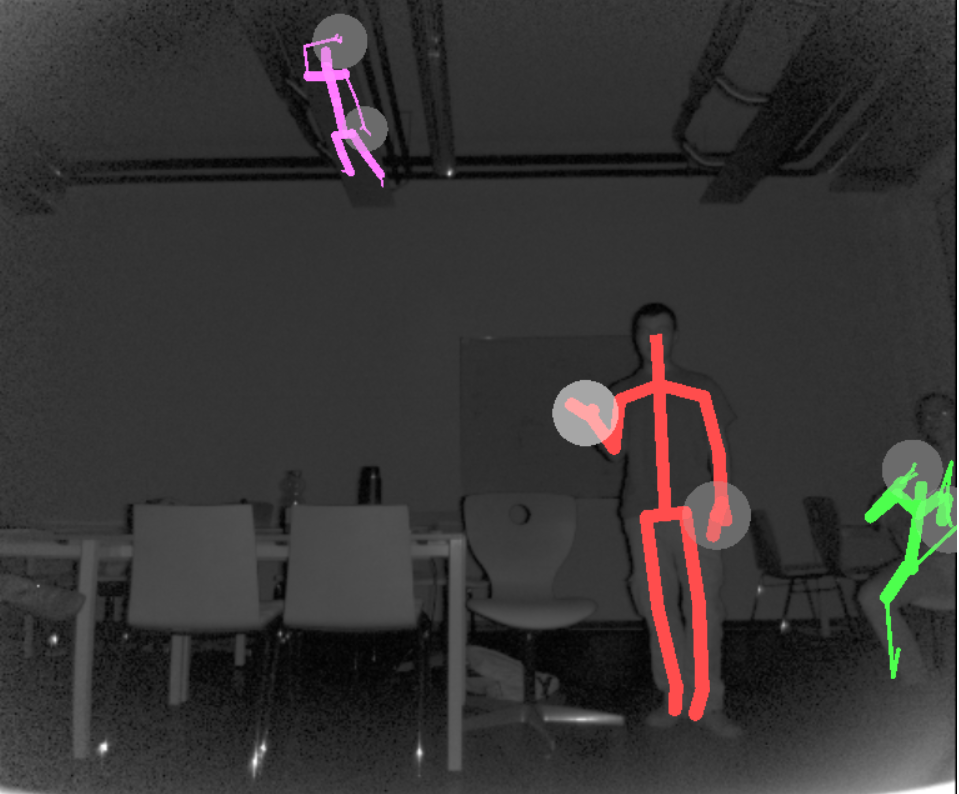
\includegraphics[width=.7\textwidth]{pictures/ninja.png}
	\caption{Infrarotbild der Kinect mit Phantom (oben links entlang der Lampe erkannt). Insbesondere werden Teile des Phantoms von der Kinect mit hoher Konfidenz erkannt (verdeutlicht durch die dicken Linien).\\
	Ferner verzerrtes Skelett am rechten Rand (verursacht durch Verlassen des Aufnahmebereichs).}
	\end{figure}
	Diese Punkte können gravierende Einschränkungen bezüglich der Programmbedienbarkeit mit sich ziehen. Eine fehlerhafte Erkennung von Positionen gemäß des ersten Punktes kann zu einem gänzlichen Verlust der gegenwärtigen Position im virtuellen Raum führen: Im naiven Ansatz wird ein hoher Differenzwert zwischen den die Bewegung (oder Drehung) bestimmenden Handpositionen festgestellt, der die Stärke der Manipulation besimmt und demzufolge auch eine extrem starke Manipulation bewirkt. Bei der Arbeit mit der Objektsteuerung ist ein weiteres Fehlerszenario aufgefallen, welches man als Sonderfall dieses Punktes betrachten kann: Ist die Hand des Nutzers, mit welcher dieser das Objekt bewegt oder dreht, durch die Kinect genau im Profil zu sehen, d.\,h. die Handfläche ist bezüglich der Höhenachse 90 Grad verdreht, so kann die Kinect nicht genau erkennen, in welche Richtung sie verdreht ist (m.\,a.\,W., ob sich der Daumen vorne oder hinten befindet). Solange dies der Fall ist, kann es passieren, dass die Kinect zwischen beiden Möglichkeiten hin- und herspringt, was sich in einer plötzlichen und äußerst starken Drehung wiederspiegelt, der jedoch keinerlei bewusste Nutzereingabe zugrunde liegt.\par 
	Eine fehlerhafte Erkennung nach Punkt drei verursacht durch die vielen willkürlichen kleinen Bewegungen eine als \glqq zittrig\grqq{} wahrgenommene Steuerung der Anwendung: So nimmt ein bewegtes Objekt etwa eine Vielzahl kleiner Bewegungen bzw. Drehungen in verschiedene Richtungen vor, ohne dass der Nutzer eine entsprechende Geste präsentiert hat.\par 
	Das vorübergehende Verlieren (oder Missinterpretieren) des vorgeführten HandStates (Punkt zwei von oben) äußert sich bei der Programmsteuerung dagegen in einem Stottern, d.\,h. dass die ursprünglich fortlaufend präsentierte Geste zu den Zeitpunkten der Fehlerkennung nicht wirkt und daher z.\,B. eine kontinuierlich angedachte Bewegung mehrfach abrupt unterbrochen wird. Siehe Abb. \ref{fig:fehlerk} für eine Illustration.\par 
	Die Erzeugung eines Phantoms ist vor allem dann kritisch, wenn das Phantom aus dem augenblicklichen Master hervorgeht. In diesem Falle übernimmt das Phantom die Programmsteuerung, wodurch einerseits der eigentliche Master die Kontrolle verliert, aber auch andererseits das Programm gänzlich chaotische Bewegungen und Drehungen vornehmen könnte. Letzteres ist wegen der Mechanismen zur Gestenerkennung jedoch unwahrscheinlich, da das Phantomskelett die entsprechenden, relativ strengen Constraints  erfüllen müsste, um den Idle-Modus zu verlassen, nach seiner Erzeugung das Programm aber  sehr schnell in den Idle-Modus bringt.
	\begin{figure}
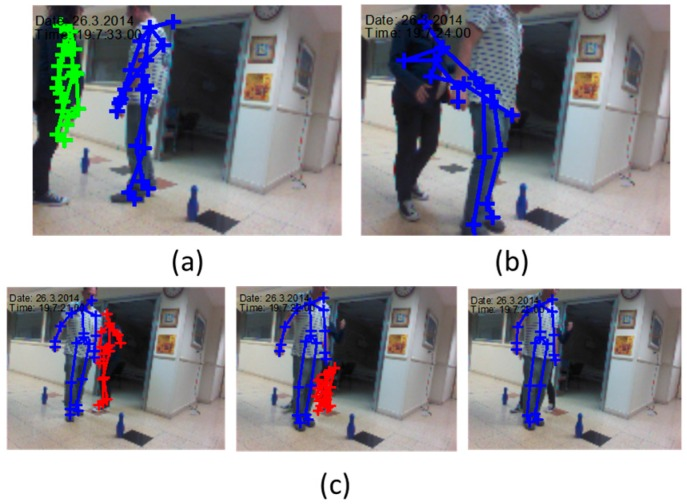
\includegraphics[width=\textwidth]{pictures/sensors-16-01965-g006.jpg}
\caption{Diverse falsch erkannte Skelette.
\begin{enumerate}[label=(\alph*)]
\item degenerierte Skelette
\item verschmolzenes Skelett
\item Skelettverlust durch Verdeckung
\end{enumerate}
Quelle: \cite{bodyprop}}
\label{fig:fehlerk}
\end{figure}
\par
	Diese Probleme üben einen negativen Einfluss auf die Erfahrung aus, die der Nutzer mit der Software macht. Insbesondere Fehler nach dem erstgenannten Schema können dem Nutzer das Erreichen seines Zieles -- etwa des Annavigierens eines Objektes -- unmöglich machen. Die weiteren Punkte werden dagegen einfach als störend empfunden. Die verschiedenen (und auch üblichen) von uns angewendeten Mechanismen, um diese Probleme zu beheben, sind weiter unten erklärt.\par
	Die genannten Schwierigkeiten ergeben sich aus den üblichen Problemen von Sensoren, wobei hier hinzukommt, dass die Kinect (wegen der primären Anwendung, die die Spieleindustrie zum Ziel hatte) über vergleichsweise preiswerte Sensoren verfügt. In diversen Arbeiten, die sich mit ähnlichen Problemstellungen beschäftigen, finden die Grenzen der Kinect nahezu durchgängig Erwähnung und ein wesentlicher Punkt in der Auseinandersetzung mit der Kinect und ihrer Anwendung in unserem und ähnlichen Szenarien widmet sich einer möglichst fehlerarmen Auswertung der qualitativ durchwachsenen Daten. In der Regel wird dabei auf Verzerrungen und schlechte Werte eingegangen, die sich durch den eingeschränkten \glqq Abdeckbereich\grqq{} der Kinect und den Einfluss von Licht ergeben (siehe \cite{bodyprop} und \cite{kinectlight}). Ferner wird darauf hingewiesen, dass das Detektions- und Trackingproblem generell von Beleuchtung, Blickwinkel, Distanz und weiteren Faktoren abhängt (vgl. \cite{thermalsens}). Ferner ist ein gerade für uns wichtiger Punkt die Abhängigkeit der Kinect-Daten von der Pose, was etwa bereits in \cite{biomid} festgestellt wurde. So ist es beispielsweise möglich, durch ungünstiges Verdecken von Körperpartien die durch die Kinect erkannten Gelenkpositionen zu verschieben. Im Test konnten wir so eine Verschiebung des Genicks (gemeint ist der Gelenkpunkt zwischen Schultern und Hals bzw. Kopf) um mehrere Zentimeter reproduzieren, indem die Hände vor dieser Stelle auf und ab bewegt werden. Besonders kritisch ist dies vor allem dann, wenn die Verdeckung nach dem Verschieben aufgehoben wird und der Gelenkpunkt an seine eigentliche Position \glqq zurückschnappt\grqq{}.
	Der ursprüngliche Ansatz, Pufferung und Mittelung, eliminiert die jitterartigen Fehler, mit denen die Kinectdaten häufig belastet sind. Hierzu wird ein Puffer vorher festgelegter Länge verwendet und während des Programmablaufs mit den für den Anwendungszweck wichtigen Daten, hier den Handpositionen des Nutzers gefüllt. Wenn unser Programm schließlich die Rückgabeparameter für die Manipulationen bestimmt, wird dieser Puffer ausgewertet. Wir bilden dabei ein exponentiell gewichtetes Mittel der gepufferten Positionen. Die neuesten Puffereinträge werden am stärksten gewichtet. Dieser Puffer dient dabei noch gleich einem anderen Zweck: Tests haben ergeben, dass das Steuern angenehmer ist, wenn die Übertragung nicht vollständig direkt von den Handpositionen erfolgt. Die Pufferlänge wurde genau so angelegt, dass das dadurch erzeugte Delay dem Nutzer nicht unangenehm auffällt und gleichzeitig die Kontrolle über das Programm per Gestensteuerung wesentlich glatter und angenehmer erfolgen kann.\par 
	Die eben beschriebene Glättung mag zwar kleine Jitterfehler ausmerzen, versagt jedoch bei Kinectdaten, die sehr stark von den eigentlichen Realdaten abweichen. Ein Beispiel für dieses immer wieder auftauchende Problem ist etwa ein weiterer Nutzer der sich im Hintergrund des steuernden Nutzers bewegt. In einem solchen Fall (und ähnlichen Fällen) kann es passieren, dass die Kinect Körperteile dieses zweiten Nutzers falsch interpretiert und dem Steuernden zuordnet. Dadurch können z.\,B. Positionsdaten entstehen, die um mehrere Meter von der Realtität abweichen. Diese Fehler benötigen eine eigene Ausreißerbehandlung: Werte, die eine zu große Abweichung von den zuletzt ermittelten Werten aufweisen (etwa eine Änderung der Handposition um mehrere Meter in aufeinanderfolgenden Frames) und daher unplausibel sind, werden auf eine vordefinierte Maximalabweichung geclippt. Ohne eine solche Behandlung hätten diese Ausreißer dazu führen können, dass der Nutzer seine aktuelle Position in der 3D-Welt ohne sein Zutun mit großer Geschwindigkeit verlässt (falls er sich etwa im Kamerabewegungsmodus befand).\par 
	Mit den gerade besprochenen Methoden haben wir also eine Reihe von Robustheitsmechanismen, was fehlerhafte Kinectdaten hinsichtlich der Position von Joints (Gelenkpunkten) angeht. Dies ist nicht der einzige Aspekt der Anwendung, der solche Sonderbehandlungen verlangt. Wir hatten oben bereits als einen derartigen Punkt die Erkennung der \glqq Hand States\grqq{} genannt. Hier ist insbesondere kritisch, dass eine Fehlerkennung nach dem ursprünglichen Modell, das nur Handzustände zu einem bestimmten Zeitpunkt diskret ausgewertet hat, zu sofortigen Zustandswechseln der Zustandsmaschine führen konnte. Besonders häufig erkennt die Kinect Handzustände in den Fehlersituationen gar nicht (und drückt dies durch \glqq Erkennen\grqq{}) des Zustands \glqq{}Unknown\grqq{} aus), teils -- wenn auch deutlich seltener -- werden jedoch auch die \glqq echten\grqq{} Zustände \glqq offen\grqq{}, \glqq geschlossen\grqq{} und \glqq Lasso\grqq{} falsch zugeordnet.\par 
	Wir wollen ferner Folgendes bemerken: Obwohl die Kinect (auch nicht intern) über keine eigenen Identifikationsmechanismen verfügt (vgl. \cite{bodyprop}), legt die durch das im SDK enthaltene Kinect Studio (siehe \cite{kinectsdk}) nahe, dass wenigstens von der Kinect mitgelieferte Konfidenzwerte für die Güte der Rückgabedaten verfügbar sind. Diese Überlegung drängte sich auf, da schlecht erkannte Gelenke (bzw. eher Gelenkverbindungen) im Studio dünner dargestellt werden, als jene, bei denen die Kinect-Daten gut zu sein scheinen: Dünne Verbindungen treten überwiegend bei Verdeckung und am Sichtfensterrand auf. Es stellte sich jedoch heraus, dass alles, was die Kinect in dieser Hinsicht bereitstellt aus drei Status pro Gelenkpunkt besteht: Jeder Gelenkpunkt ist getrackt (\glqq Tracked\grqq), nicht getrackt (\glqq NotTracked\grqq) und vermutet (\glqq Inferred\grqq). Über den letzten Status ist der Dokumentation (siehe \cite{trackingstate}) nur zu entnehmen, dass das Vertrauen in die Richtigkeit der Daten \glqq sehr gering\grqq{} ist.\par\bigskip
	Abschließend sei noch ein Szenario genannt, gegen das unsere Robustheitsmechanismen keinen hinreichenden Schutz bieten: Das der gezielten Manipulation. Wie bereits bemerkt, sind die Kinectdaten z.\,T. ungenau, etwa bezüglich der Gelenkpositionen. Durch (gegebenenfalls bewusstes) Verdecken oder Unkenntlichmachen von Körperteilen ist es möglich, die von der Kinect erkannten Jointkoordinaten zu verschieben. Dies kann durch den Einsatz von der Hände und der Körperhaltung, aber auch z.\,B. durch weite Kleidung hervorgerufen werden. Wir erklären das Problem an einem Beispiel: In unserer Mastererkennung verwenden wir neben anderen Körpermerkmalen etwa die Torsolänge. Ein Nutzer, der von der Kinect getrackt wird, kann jedoch die an ihm erkannte Torsolänge (genauer den Abstand zwischen den entsprechenden erkannten Gelenkpunkten) verändern, indem er sich beispielsweise streckt und \glqq groß macht\grqq{} (dies verlängert die erkannte Torsolänge) oder aber sich leicht nach vorne beugt (was die erkannte Torsolänge staucht). Dies eröffnet ihm einen Spielraum bezüglich des genannten Merkmals, in dem er die vom eingespeicherten Master bekannte Torsolänge annähern kann. Ähnliches ist für andere Körperteile reproduzierbar, etwa durch leichtes Beugen der Arme oder Anheben und Hängenlassen der Schultern. Eine weitere, aber weniger relevante Möglichkeit ist auch das Ausnutzen von Kinect-Ungenauigkeiten am Rande ihres Aufnahmebereiches, z.\,B. weit weg von der Kamera. Ihre kleinere Relevanz liegt in der Schwierigkeit begründet, \emph{bewusst} diverse Effekte hervorzurufen, da die Randungenauigkeiten aus Anwendersicht willkürlich und ohne Muster sind.\par
	Für Nutzer, die sich ohnehin aufgrund ihrer Körpermerkmale recht ähnlich sind, ist es bei solchen wie eben beschriebenen Manipulation schließlich nicht mehr sicher möglich, eine korrekte Entscheidung zu fällen. Es sei jedoch noch einmal darauf hingewiesen, dass der Beeinflussungsspielraum relativ gering und damit nur für a priori ähnliche Skelette von Belang ist. Ferner ist es augenscheinlich unmöglich, die Manipulation ohne Debugausgaben der genauen Werte bewusst und gezielt durchzuführen.
